\documentclass{beamer}
\usepackage{graphicx}
\usetheme{metropolis}

\title{Enabling Text Analytics}
\author{Jason Cairns}
\institute{University of Auckland}
\date{November 20, 2019}
% \logo{
\includegraphics[height=2cm]{img/uoalogo.png}}

\begin{document}

\maketitle{}

\begin{frame}
  \frametitle{Introduction}
  \begin{itemize}
  \item The intention of this project is to develop a user friendly
    program that that allows for the performance of common text analyses.
  \item It is intended to be capable of integrating with iNZight, with a
    similar user base.
  \item The application is to be flexible enough to deal with a range of
    text formats, and produce attractive output quickly.
  \end{itemize}
\end{frame}

\begin{frame}
  \frametitle{Text Analytics}
  \begin{itemize}
  \item Text Analytics is comprised of a variety of processes and techniques
to extract information from text and provide a high-level overview.
\item The text almost always requires some initial processing.
  \begin{description}
  \item[Lemmatisation]
  \item[Stopwords] 
  \item[Sentiment]
  \item[Associated Words]
  \item[Summarisation] 
  \end{description}
  \end{itemize}
\end{frame}

\section{Program Description}

\begin{frame}
  \frametitle{Development Areas}
  \begin{description}
  \item[Processing] 
  \item[Insight] 
  \item[Visualisation] 
  \end{description}
\end{frame}

\begin{frame}
  \frametitle{Program Architecture}
  \begin{figure}
  \centering 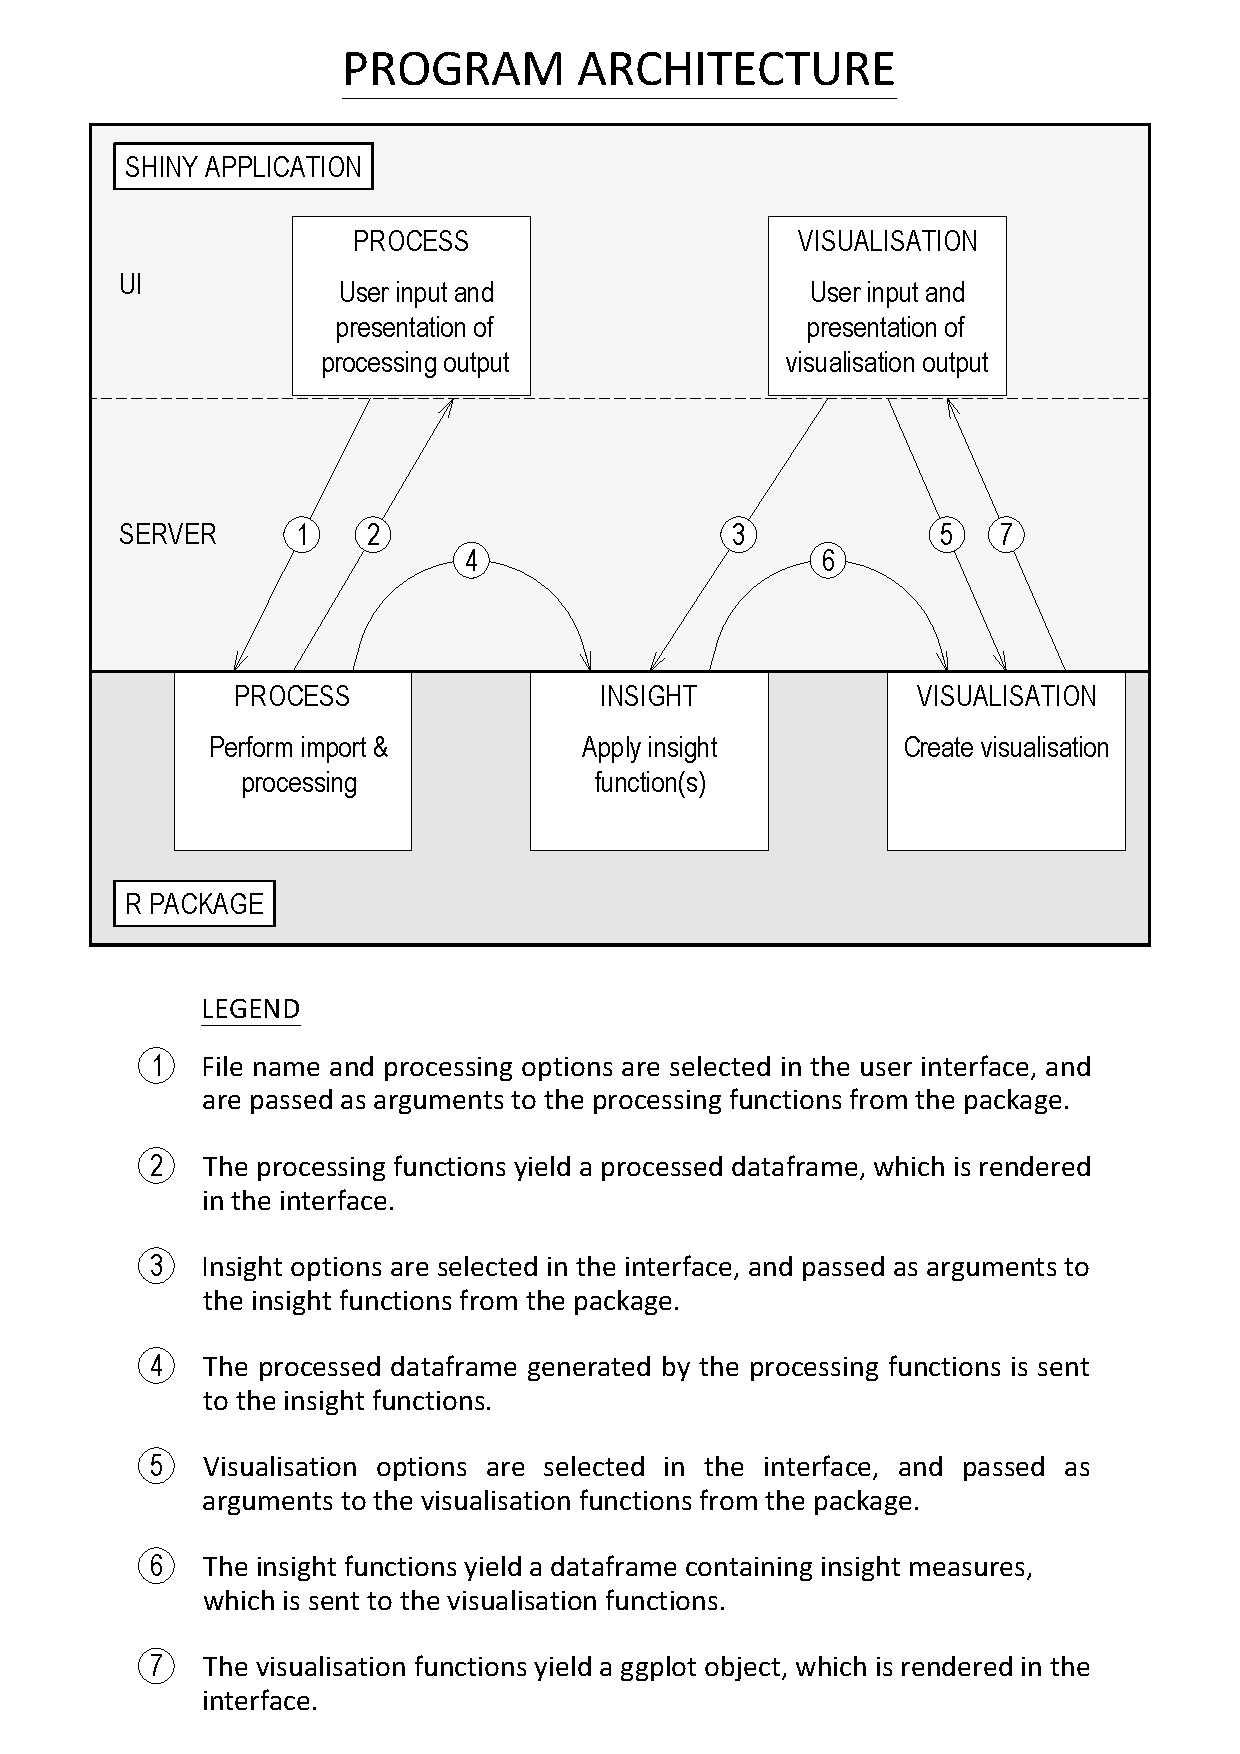
\includegraphics[scale=0.4]{img/arch-expanded.pdf}
  \caption{Program architecture\label{fig:pr-arch}}
\end{figure}
\end{frame}

\end{document}